\setchapterpreamble[u]{\margintoc}
\chapter{Artistic Computer Vision}
\labch{ACV}
This chapter shall dive into existing and related work that combines computer vision with artistic content.

Applying computer vision techniques to images with artistic content has been interesting and challenging at the same time.
Due to the often observed change in appearance that can be observed for many artistic images, existing CV pipelines for \ie classification usually do not work as intended.
This makes it all the more interesting to see, how these pipelines are affected by this domain gap.

At the same time artistic images bring something into the mix which 

%non-photorealistic rendering vs. photrealism
%clesly realted to texture synthesis and transfer
%games and movies benefit from this
%since the 1990's starting with artistic rendering of images (paint by numbers)

%with neural network more practical applicatin of style transfer have become popular:
% - funny iphone filters
% - translating images between other domains (google maps, satelites etc.) -> many possible applications
% quantitative style (materials used, color shoice etc.)
% qualitative style (how are people drawn etc.)

% historically there have been many different approaches
%try to group these approaches on the problem formulation and the approach

%color choice
%how to display something (is it unnaturally large or small ...)
%direction of brush strokes
%choice of material
%which details are kept which details are lost?

%all of this together makes style

%usually style transfer formulates this much simpler (maybe see gatys formulation?):
%create something that maintains the orginal content to some  degree but people would categorize together with other works of that 'style'
% style is rather something by what art can be grouped together 'easily'


\section{Problem Formulation \& Approach}
The problem that style transfer might seem easy to capture at first, but it quickly becomes harder when trying to formulate it.
As 'style' is simply defined as "a typical way of doing something", it includes actually all aspects 

%style transfer
%create IMAGE that catches style as well a possible, doesn't rally matter how, the pixel should make sense in the end

%painterly rendering
%create something that looks like is has been drawn with a paint brush (or any other such tool, e.g. has some gloss to it etc.)
%don't really concentrate on deeper style but just the apprearance

%drawing networks
%do not care as much about the apprearance or the style but how to compose the image in a different parameter space, FAST

%brush stroke extraction and image analysis
%get more information about the image, that can help to classify it, or identify it. Do not get all brush strokes but those that are characteristic

%drawing networks and painterly rendering are really much of the same with different focus on what matters.


%this work would fall into painterly rendering territory paired with brush stroke extraction


%features of DNN have been used to classify paintings

\section{Brushstroke Extraction}
%no updates in recent years
%relatively small field
%shift towards creating art rather than analyzing it
%what to do with the data besides identifying forgeries?


\section{Painterly Rendering}
\labsec{PR}

%refer to painterly rendering review

Painterly rendering or stroke-based rendering is a field of computer vision that tries to achieve stylization of images by reconstructing them with hard regularization. 
One such regularization could be using only cycles or other geometric shapes..

This limits the reconstruction's faithfulness but add a layer of abstraction that stylizes the image as well.
Painterly rendering is seldomly included into the field of style transfer (which shall be explained in the next section) as there is not really target 'style', as it is usually understood.
As the goal is always just reconstruction an image as good as possible with the regularization at hand the target style can only formulated very broadly, like 'pointillism' or 'painting'.
Any control over the painting beyond that is really hard to realize.

On the other side, the resulting representation can come in a parametrized form, such that the image can be brought into a different domain.

\subsection{Genetic Algorithms}
Genetic algorithms are typically not closely associated with painterly rendering, even though they represent just a different approach to algorithms for this problem.

Genetic algorithms already perform a similar task in order to approximate images by other geometric shapes or even smaller photos (also known as the popular photo mosaic effect).
\paragraph{Genetic algorithms} follow a random sampling approach that 'evolves' as genomes do.
Starting with a random set of circles that are parameterized by their position, radius, and color, it then chooses the most successful samples and resamples in a region around these.
This process is repeated until a certain level of convergence is reached.


\subsection{Stroke-Based rendering}

%refer to neural style transfer: a review

\begin{marginfigure}
    \includegraphics{genetic_starry_night}
    \caption[]{Starry Night approximated by a genetic algorithm using only circles. \url{https://effyfan.com/2018/03/02/w6-van-gogh-flowfield/}}
    \labfig{genetic}
\end{marginfigure}

As well as this does work, it is very much computationally expensive as most samples will not fit the image, thus searching for the small set of fitting shapes requires to evaluate all the wrong shapes as well.
Considering artworks, brushstrokes have many more degrees of freedom, and artworks usually consist of upwards of a few thousand brushstrokes.
Consequently, it would be considerably more challenging to apply to this problem until computational resources have become a few magnitudes more powerful.

\begin{figure}
    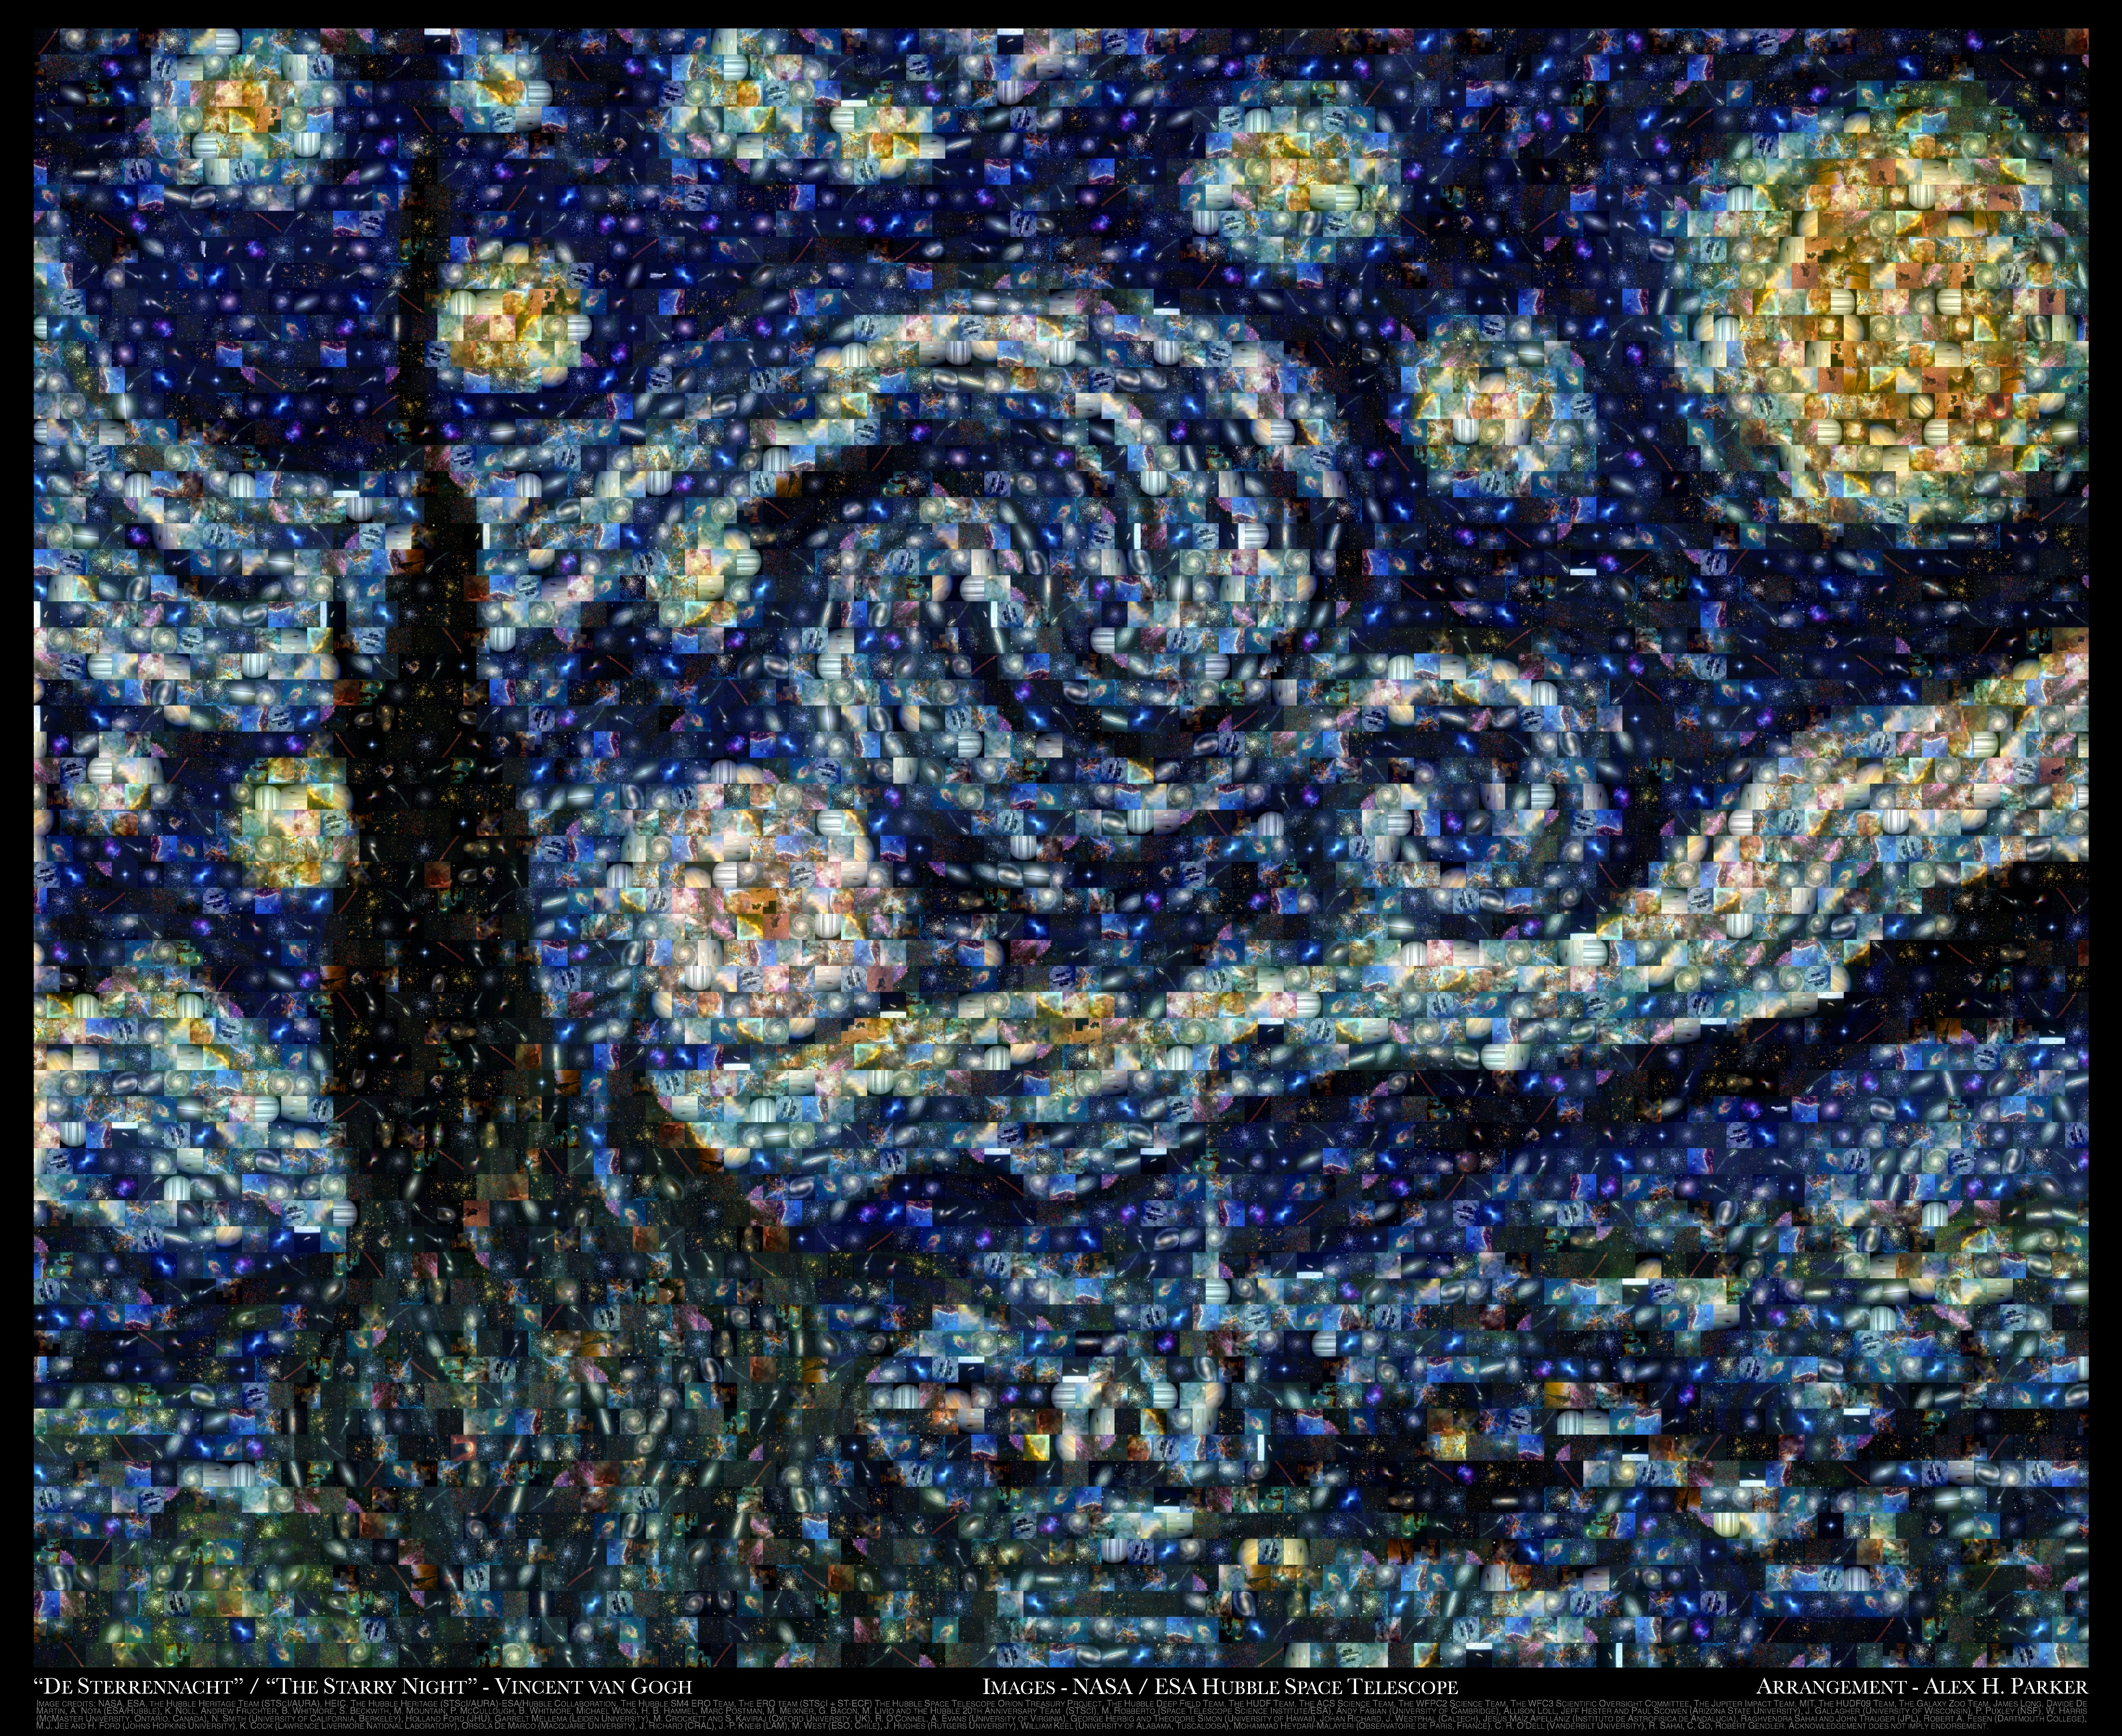
\includegraphics{photomosaic_starry_night}
    \caption[]{Photo mosaic of Starry Night using only images by the Hubble Space Telescope. \url{http://www.astro.uvic.ca/~alexhp/new/figures/starrynight_HST.001.jpg}}
    \labfig{photomosaic}
\end{figure}

\section{Style Transfer}
\labsec{ST}

This field of style transfer has its origins 
%most active field
%style and texture are similar problem

\subsection{Early Approaches}
Earliest approaches
%painterly rendering is some kind of style transfer but shall be dealt with explicitly
%focus is on approaches that work only with pixels
%filters
%texton based approaches

%Some early approaches include histogram matching on linear filter responses [19] and non-parametric sampling [12, 15].
%       . Pyramid-based texture analysis/synthesis
%       Split and match: example-based adaptive patch sampling for unsupervised style transfer
%       Image quilting for texture synthesis and transfe
%low-level statistics and fail to perceive semantic structures



\subsection{Neural Style Transfer}
%A bit similar to transfer learning -> utilize the pretrained features especially of the early layers.
The field of style transfer has really gained traction in 2015 with the publication of \textbf{A Neural Algorithm for Artistic Style} by \citeauthor*{gatys}.
It was the first approach to transfer the style of one image to another and at the same time maintaining a high contextual fidelity.
In retrospective, this work really kicked off neural style transfer as a field.

\citeauthor*{gatys} themselves pinpoint the novelty of their approach as 'manipulations in feature spaces' as opposed to previous approaches that 'directly manipulate the pixel representation of an image'\cite{gatys}.
They use existing neural architectures and extract information in two separate ways, such that content and style can be separated.

Previous works already used \textbf{perceptual loss} to accumulate information on the content in an image \cite{percep_loss}, or check whether two images have the same content \cite{other_percep_loss}.
%networks trained on object recognition increasingly care about the content with every layer
Perceptual loss is based on the VGG-19 architecture \cite{VGG} which is a deep CCN trained for object classification on ImageNet \cite{imagenet}.
By arguing that the network's layer activations increasingly respond to the content when following the networks' hierarchy.
Some much even, that it is possible to reconstruct the content of an image by using the activations of one such layer.

For reconstruction of an image's content, gradient descent is performed on a white noise image.
The gradient descent aims to minimize the perceptual distance between the reconstruction and the target image.
Perceptual distance is defined as the L2-distance between the activations of two images in deep layer of the VGG-network.

For image vector $\vec{x}$ with $\vec{x} \in = \R^{M_0}, M_0 = H_x \dot W_x $, a layer $l$ of the network has $N_l$ feature maps of size $M_l$.
In this case $M_l$ is equal to the height times the width of the feature map of the $l$-th layer.
The activations of the $i$-th filter ($i \in N_l$) at position $j$ ($j \in M_l$) at layer $l$ can then be represented by matrix $F(\vec{x})_{ij}^l \in \R^{N_l \times M_l}$.
The perceptual distance is then defined as
\begin{align}
    d_{\text{percep}}(\vec{x}, \vec{y}) = \sum_{i, j} (F(\vec{x})_{ij}^l - F(\vec{y})_{ij}^l)^2 = \norm{\tensor{F(\vec{x})}^l - \tensor{F(\vec{y})}^l}_2^2
\end{align}
, which allows to define the perceptual loss or content loss as 
\begin{align}
    \L_{\text{content}} = \frac{1}{2} \sum_{i, j} (F(\vec{x})_{ij}^l - F(\vec{y})_{ij}^l)^2 = \frac{1}{2} \norm{\tensor{F(\vec{x})}^l - \tensor{F(\vec{y})}^l}_2^2
\end{align}

\marginnote{The factor $\frac{1}{2}$ will cancel out when deriving $\L_{\text{content}}$ with respect to $F(\vec{x})_{ij}^l$.}

Minimizing the content loss between two images, by using gradient descent the content of an image can be restored (see \reffig{content_style_loss}).

\begin{figure*}
    \includegraphics{content_style_loss}
    \caption[]{Reconstructions of content(bottom) and style(top) using different layers. \cite{gatys}}
    \labfig{content_style_loss}
\end{figure*}

As approximating the content of an image has now become possible, the question is whether this is possible with style as well.
\citeauthor*{gatys} again turned to the pre-trained VGG network for this.
They explicitly reduce style to texture for this reason and thus search for a feature space that captures \textbf{texture} rather than content.
Subsequently, \citeauthor*{gatys} propose the use of \textbf{Gram matrices} as they capture the correlations of feature-activations over their spatial extent.

The Gram matrix of a given matrix $\tensor{A}$ is the inner product of all column vectors in $\tensor{A}$.
\begin{align}
    G = \langle a_{i}, a_{j} \rangle = \tensor{A}^T \tensor{A} \text{ if $a_1$...$a_j$ are column vectors of $\tensor{A}$}
\end{align}
The resulting Gram matrix G now has the form $j \times j$ and captures texture information but no longer the global content.

\refsec{problem} already mentioned that style is very complex and exists at various scales at the same time which \citeauthor*{gatys} address by using many layers.
As these layers sit at different depths their field of view varies and each layer captures information at a different scale.
Early layers will tend to hold small scale information, later layers will hold larger scale information with every layer.

\citeauthor*{gatys} first compute the Gram matrices each layer $l$ for both the target style image and the current image.
Then they use the L2 distance metric to measure the discrepancy between them.
\begin{align}
    G(\vec{x})^l & = \frac{1}{(2 N_x^l M_x^l)^2} F(\vec{x})^l{}^T F(\vec{x})^l \\
    G(\vec{y})^l & = \frac{1}{(2 N_y^l M_y^l)^2} F(\vec{y})^l{}^T F(\vec{y})^l \\
    d_{\text{style}}^l(\vec{x}, \vec{y}) & = \norm{G(\vec{x})^l - G(\vec{y})^l}^2_2 \\
\end{align}

\marginnote{The denominator of $\frac{1}{4 N_x^l{}^2 M_x^l{}^2}$ is squared since the Gram matrix is the product of a matrix with itself transposed.}

The style distances at each layer are then weighted and summed up to make up the style loss:

\begin{align}
    \L_{\text{style}} = \sum_{l} w_l d_{\text{style}}^l(\vec{x}, \vec{y})
\end{align}

%again one can visualize the style/texture that is perceived
This style loss can again by used together with gradient descent in order to check whether it is possible to reconstruct the texture of an image much like the content of an image.
\reffig{content_style_loss} shows that it is in fact possible to reconstruct the texture of the image at various scales.
Specifically the local consistency of each texture becomes larger, the deeper the layer sits.

%mix content and style
\citeauthor*{gatys} now combine the losses for one content image $\vec{c}$ with a style image $\vec{s}$ and optimize $\vec{x}$ in the same way the reconstructions have been obtained.

\begin{align}
    \L_{\text{total}} = \lambda_{\text{content}} \L_{\text{content}}(\vec{x}, \vec{c}) + \lambda_{\text{style}} \L_{\text{style}}(\vec{x}, \vec{s})
\end{align}

\begin{marginfigure}
    \includegraphics{gatys_ST}
    \caption[]{Style transfer examples by \citeauthor*{gatys}. \cite{gatys}}
    \labfig{content_style_loss}
\end{marginfigure}

The result of this can be seen in \reffig{gatys_ST}

\subsubsection{Follow-Up Research}
There has been some follow-up research on \citeauthor*{gatys}'s work which addresses mainly how the style loss works.

\citeauthor*{MMD} have shown that the style loss is equivalent to calculating the \textbf{maximum mean discrepancy (MMD)} between the features of each layer \cite{MMD}.
MMD is a test-statistic for a null hypothesis $p=q$ with the data $X = \{x_i\}^n_{i=1}$, sampled from $p$, and $Y = \{y_i\}^n_{i=1}$, sampled from q, at hand.
It can be used as a difference measure as well and vanishes only if $p=q$.
\begin{align}
    \text{MMD}^2[X, Y] & = \frac{1}{n^2} \sum^n_{i=1} \sum^n_{i'=1} k(\vec{x}_i, \vec{x}_{i'}) \\
    & + \frac{1}{m^2} \sum^m_{j=1} \sum^m_{j'=1} k(\vec{y}_j, \vec{y}_{j'}) \\
    & - \frac{2}{nm} \sum^n_{i=1} \sum^m_{j=1} k(\vec{x}_i, \vec{y}_{j})
\end{align}

MMD can be based on different kernel functions $k$ and \citeauthor*{MMD} have shown that the style loss is equivalent to the squared MMD with a polynomial kernel.
Consequently they were able to show, that style transfer work with different kernel functions as well and even by explicitly matching the batch statistics (see \reffig{MMD}):
\begin{align}
    d_{\text{style}}^l(\vec{x}, \vec{y}) & = \frac{1}{N_l} \sum_{i = 1}^{N_l} \left( (\mu^i_{F(\vec{x})^l} - \mu^i_{F(\vec{y})^l}) + (\sigma^i_{F(\vec{x})^l} - \sigma^i_{F(\vec{y})^l}) \right)
\end{align}

\begin{figure}
    \includegraphics{MMD}
    \caption[]{Reconstructed textures for Starry Night using different kernel functions $k$ \cite{MMD}}
    \labfig{MMD}
\end{figure}


\citeauthor*{LenDu} tested whether pre-trained weights play an important role when performing style transfer.
He was able to show basic style transfer even with random initialized networks, but results vary wisely depending on the random initialization.
Ultimately, it is possible so obtain some style transfer with this technique but the pre-trained weights seem to play an important role in stablizing the reconstruction process.

\subsection{State of the Art}

\subsubsection{Real-Time Style Transfer}
%johnson
Following \citeauthor*{gatys} seminal work, other have followed suit in trying to stylize images with neural networks.
\citeauthor*{Johnson} were the first to use the same losses but train a feed-forward architecture with it \cite{johnson}.
They were able to significantly speed up the stylization process like this as stylization was performed in a single feed-forward pass instead of a lengthy gradient descent optimization.
Ultimately, this enabled them to generate stylized images in real-time from a given content image, using a deep residual convolutional neural network.
\begin{figure*}
    \includegraphics{johnson_net}
    \caption[]{Training set-up by \citeauthor*{johnson}. \cite{johnson}}
    \labfig{johnson_net}
\end{figure*}

%markov random field ansatz?

%adain
\subsubsection{Arbitrary \& Universal Style Transfer}
\citeauthor*{AdaIN} used a different feed-forward approach for arbitrary style.
They first encode an arbitrary style image $\vec{s}$ as well as a content image $\vec{c}$ using a pre-trained VGG network.
This allows them to obtain the activations at a very deep layer of the network $F^l(\vec{s})$ and $F^l(\vec{c})$.
Then they compute the second order statistics for both $\mu_F^l(\vec{s}), \sigma_F^l(\vec{s})$ and $\mu_F^l(\vec{c}), \sigma_F^l(\vec{c})$.
Using adaptive instance normalization (AdaIN), they rescale the content activations such that they match the statistics of the style activations.
\begin{align}
    F'^l = \sigma_F^l(\vec{s}) \frac{F^l(\vec{c} - \mu_F^l(\vec{c})}{\sigma_F^l(\vec{c})} + \mu_F^l(\vec{s}) 
\end{align}
Finally, they train a decoder that minimizes the style and content loss, as they have been proposed by \citeauthor*{gatys}.
They achieve comparable results to other style transfer approaches at a similar speed to \citeauthor*{johnson} while allowing for any target style eventhough only training only once.
\begin{figure*}
    \includegraphics{adain_net}
    \caption[]{Training set-up by \citeauthor*{AdaIN}. \cite{AdaIN}}
    \labfig{johnson_net}
\end{figure*}

%wct
\todo{this is actually just PCA decompsition to a certain degree}
A similar approach by \citeauthor*{WCT} relies on matching the covariance and the mean of content and style activations.
They do that through what they call 'whitening and coloring transform' \cite{WCT}.
First they whiten $F^l(\vec{c})$ into $\hat{F}^l$ such that $\hat{F}^l \hat{F}^l{}^T = I$
\begin{align}
    \hat{F}^l = E_c D_c^{-\frac{1}{2}} E_c^T (F^l(\vec{c}) - \mu_c)
\end{align}
Where $D_c$ is the diagonal matrix of eigenvalues of the covariance matrix and $E_c$ is the respective orthogonal matrix of eigenvectors.
such that
\begin{align}
    F^l(\vec{c}) F^l(\vec{c})^T = E_c D_c E_c^T
\end{align}

Then coloring is performed by rescaling the whitened representation $\hat{F}^l$ into $\tilde{F}^l$
\begin{align}
    \tilde{F}^l = E_s D_s^{\frac{1}{2}} E_s^T \hat{F}^l + \mu_s \\
    F^l(\vec{s}) F^l(\vec{s})^T = E_s D_s E_s^T
\end{align}

The resulting $\tilde{F}^l$ is then decoded with a pre-trained decoder to render the final stylized result.
\citeauthor*{WCT} use pre-train the decoder solely on natural images and perceptual loss and reconstruction loss as objective.
Additionally, they introduce a pipeline that performs style transfer on multiple scales sequentially.
They achieve good results in real-time with just training the decoder once.

\subsubsection{Bidirectional Style Transfer}
%cyclegan
\citeauthor*{CycleGAN} went a different way on style transfer and rely on a generative adversarial objective to identify style in an image.
Specifically, they transform images between any two domains $x \in \mathcal{X}$ and $y \in mathcal{Y}$, not just photos and artworks.
For this, they use two discriminators ($D_X$ and $D_Y$, one for each domain) as well as two transformation networks ($G: X \rightarrow Y$ and $H: Y \rightarrow X$).
Each translation network then transforms a given sample from one domain into the other and the discriminator assesses the result.

\begin{align}
    \L_{\text{adv}} = \log D_Y(y) + \log(1 - D_Y(G(x)))
\end{align}

Additionally, the transformed image is then transformed \textit{again} and compared to the original input, in what they call \textbf{cycle loss}.

\begin{align}
    \L_{\text{cycle}} = \norm{F(G(x)) - x}^2_2
\end{align}

In the end, \citeauthor*{CycleGAN} are able to stylize and de-stylize images with their networks $G$ and $H$.
The main novelty here though is the good stylization quality they achieve without any of the previously introduces style losses.
They have also shown one way, in which GANs are also capable of performing style transfer reasonably well.
Other notable efforts were \todo{list GAN-based style transfer efforts}.

\subsubsection{Adversarial Style Transfer}
Building on these GAN-based approaches, \citeauthor*{artsiom} improved the quality of adversarial style transfer and extended it to abstract styles as well.
They argue that ImageNet-based approaches inherently favor photorealistic styles through the data set that ImageNet has been trained on \cite{artsiom}.
Furthermore, approaches like cycleGAN suffer a similar fate as the back-transformation with cycle consistency opposes loss of detail in more abstract styles.

In order to retain content and global structure of an image, they introduce a fixed-point loss, which requires the stylized image to stay as-is when being re-stylized.
\begin{align}
    \L_{\text{content}} = \norm{E(G(E(x))) - E(x)}^2_2
\end{align}
To minimize this loss, the encoder must understand original content and stylized content.
They also implement a transformed reconstruction loss for better visual quality of the stylized image
\begin{align}
    \L_{\text{transformed}} = \norm{T(x) - T(G(E(x)))}^2_2
\end{align}
The results show good visual quality, especially concerning the details and loss of details for abstract styles.
Also this approach focusses on stylizing not only for a single image but the style of an artist in general.

\citeauthor*{dima} take this further and focus on stylizing different content specifically.
This means, a person is differently depicted than a tree, considering level of detail, colorscheme \etc. , which holds with real-world experience.
They achieve this by using the same fixed-point loss that \citeauthor*{artsiom} but combine it with a second update step.
In this second update step they require similar scenes to be placed closely in feature space and dissimilar scene to lie further apart.
They add a transformation block between encoder and decoder shape the feature space accordingly.

\subsubsection{Others}
There exist many other approaches that are capable of transferring style.
Some focus very heavily on stylization of portraits using self-attention modules \cite{ugatit}.
Others choose an approach similar to cycleGAN but add a shared encoding space for content and separate attribute spaces where style is encoded \cite{unit, munit, drit, drit++}.
With the latter ones mainly focussing on separating shape and appearance of images and recombining them arbitrarily.
One such example is taking the posture of a person in one image and combining it with the clothes and appearance of a person in another image.

The lines between these the applications and style transfer as it has been presented are blurry with many approaches that are capable of performing both.


\section{Drawing Networks}
%gaining traction

%learning2Paint
%SPIRAL
%DrawNet
%PaintNet


%image transofrmation tasks denoising, colorization, super-resolution, semantic-segmentation, depth estimation, 
